% Provenance (never printed): old terminale S material on the continental crust
% (granitic composition, thickness, density, age; roots and isostasy). Thickness
% from Christensen-Mooney 1995 and Cogley 1984 (CRUST1.0 dropped: no licence,
% Sync 1); ocean-floor ages from figdata/grade-12/crust_ages.py (Seton 2020 grid,
% as in g11.01). Airy isostasy is g11.03's: recalled, not re-derived. Radiometric
% dating is g12.07's: ages are only quoted here.
\chapter{大陆地壳}\label{ch:g12:continental-crust}

在加拿大西北部阿卡斯塔河附近，出露一种灰色岩石，
其上有浅色与深色条带。该岩石的年龄测定为 40.0 至 40.3 亿
年，即阿卡斯塔片麻岩，是已知最古老的岩石。更古老的是
矿物锆石的颗粒，每颗仅几分之一毫米长，见于古老的
澳大利亚西部杰克山的沉积岩中。这些锆石由更老的岩石
剥蚀而来，经水搬运后才被埋藏，它们结晶于 44
亿年前，这表明当时已有地壳。任何洋底的年龄都不足它的二十分之一。
本章探讨大陆由什么构成，以及它们为何能长久留存。
% ledger: bowring99:acasta, wilde01:zircon, uw14:jack-hills, photo:g12-acasta, photo:g12-jack-hills-zircons

\begin{omfigure}
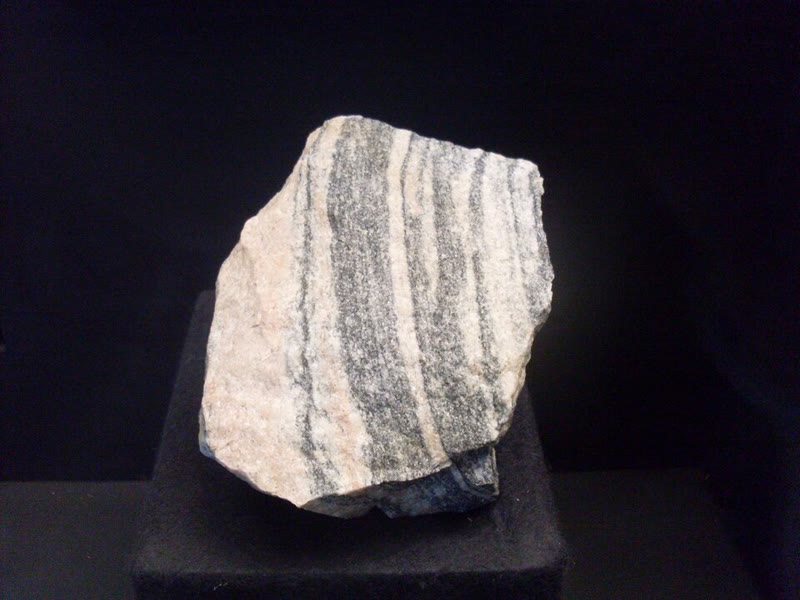
\includegraphics[height=4.6cm]{images/book2/g12-pedro-acasta-gneiss.jpg}\hspace{0.04\linewidth}%
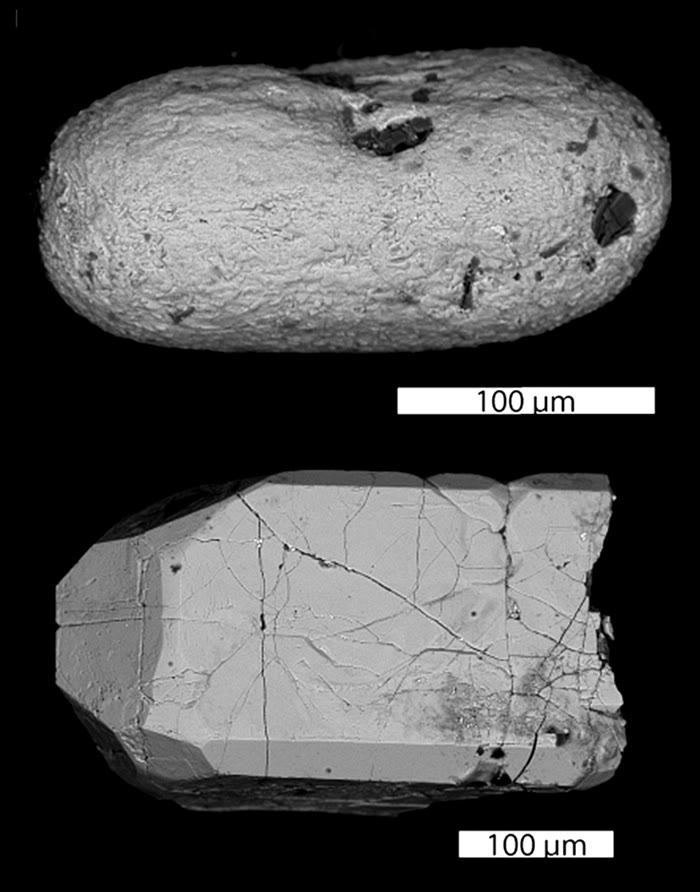
\includegraphics[height=4.6cm]{images/book2/g12-cavosie-jack-hills-zircons.jpg}

{\small 左：一块阿卡斯塔片麻岩标本，年龄 40.3 亿年，陈列于
博物馆展柜中。照片：Pedroalexandrade（CC~BY-SA~3.0）。右：澳大利亚西部杰克山的两颗
锆石颗粒，用电子
显微镜观察；每条比例尺长 \qty{100}{\micro m}。上方颗粒在
被水搬运时已磨圆，下方颗粒保留了晶面。
图片：A.~Cavosie 与 J.~Valley（公有领域）。}
\end{omfigure}
% ledger: photo:g12-acasta, photo:g12-jack-hills-zircons

\begin{recall}
地壳以\omterm{def:g11:seismic-structure:moho}{莫霍面}为下界，其下是密度更大的地幔
（见\cref{ch:g11:seismic-structure}）。大洋地壳厚约 \qty{7}{km}，
由在洋中脊形成的玄武岩和\omterm{def:g11:ocean-ridges:gabbro}{辉长岩}组成（见\cref{ch:g11:ocean-ridges}）。
其年龄从不超过约 1.9 亿年（见\cref{ch:g11:drift-to-spreading}）。
\omterm{def:g11:lithosphere-asthenosphere:lithosphere}{岩石圈}外层漂浮于\omterm{def:g11:lithosphere-asthenosphere:lithosphere}{软流圈}之上。按艾里模型，凡
地面高出 $h$ 的区域，地壳增厚 $h\,\rho_m/(\rho_m -
\rho_c)$（见\cref{ch:g11:lithosphere-asthenosphere}）。火成岩按
\omterm{def:g11:igneous-rocks:texture}{结构}和二氧化硅含量命名：\omterm{def:g11:igneous-rocks:felsic-mafic}{镁铁质}岩为 45 至
\qty{55}{\percent} \ce{SiO2}，\omterm{def:g11:igneous-rocks:felsic-mafic}{中性}为 55 至 65，\omterm{def:g11:igneous-rocks:felsic-mafic}{长英质}为 65 至
75（见\cref{ch:g11:igneous-rocks}）。放射性元素以稳定的
速率衰变，由此可确定岩石的年龄（物理学相关分册；
见\cref{ch:g12:age-of-the-earth}）。
\end{recall}
% ledger: white92:crust, data:b2-seafloor-age, tulane:magma-types

\section{大陆由什么构成}

\begin{definition}[大陆地壳]\label{def:g12:continental-crust:continental-crust}
称\emph{大陆地壳}\index{大陆地壳}为构成大陆的地壳，
包括位于浅海之下的部分。其
厚度大，上部平均为花岗质成分，质轻，
并且可以非常古老。
\end{definition}
% ledger: tulane:crust-types, tulane:roots, cogley84:continents

大陆的范围比陆地更大。\omterm{def:g12:continental-crust:continental-crust}{大陆地壳}的边缘
延伸至海下，位于大陆架上：按此方式划定，\omterm{def:g12:continental-crust:continental-crust}{大陆地壳}
覆盖面积为 2.1 亿~\unit{km^2}，占地球
表面的 \qty{41}{\percent}，其中将近三分之一，\qty{30.6}{\percent}，
被海水淹没。计入海下部分后，\omterm{def:g12:continental-crust:continental-crust}{大陆地壳}的
平均高度仅约 \qty{120}{m}，高于海平面。
% ledger: cogley84:continents

地表的大陆可见各类岩石——沉积物、
\omterm{def:g11:igneous-rocks:volcanic-plutonic}{火山岩}、变质岩——但在沉积\omterm{def:g11:fossil-fuel-geology:reservoir}{盖层}之下，\omterm{def:g12:continental-crust:continental-crust}{大陆地壳}
主要由花岗质岩石，以及老造山带根部的变质岩和
\omterm{def:g11:igneous-rocks:volcanic-plutonic}{深成岩}构成。平均而言，整个\omterm{def:g12:continental-crust:continental-crust}{大陆地壳}含
二氧化硅 \qty{60.6}{\percent}；其上部更富，
为 \qty{66.6}{\percent}，因此深部必定较贫。
% ledger: rg14:crust, tulane:crust-types, cm95:crust

\begin{omfigure}
\begin{tikzpicture}
\begin{axis}[omrecord, ybar=0pt, width=0.92\linewidth, height=5.0cm, bar width=7pt,
  ymin=0, ymax=80, ylabel={质量分数（\unit{\percent}）},
  symbolic x coords={SiO2, Al2O3, FeO, MgO, CaO, Na2O, K2O},
  xticklabels={\ce{SiO2}, \ce{Al2O3}, \ce{FeO}, \ce{MgO}, \ce{CaO}, \ce{Na2O}, \ce{K2O}},
  xtick=data, enlarge x limits=0.08, ymajorgrids=true, xmajorgrids=false,
  legend style={font=\scriptsize, at={(0.98,0.97)}, anchor=north east, legend columns=1}]
% ledger: rg14:crust (upper and bulk continental crust; FeO* total iron)
\addplot[fill=omLithGranite, draw=black!60] coordinates {(SiO2,66.6) (Al2O3,15.4) (FeO,5.04) (MgO,2.48) (CaO,3.59) (Na2O,3.27) (K2O,2.80)};
\addplot[fill=omProp!55, draw=black!60] coordinates {(SiO2,60.6) (Al2O3,15.9) (FeO,6.71) (MgO,4.66) (CaO,6.41) (Na2O,3.07) (K2O,1.81)};
% ledger: earle:magma-oxides (mafic magma: midpoint of each range, the bar spans the range)
\addplot[fill=omLithBasalt, draw=black!60, error bars/.cd, y dir=both, y explicit]
  coordinates {(SiO2,50) +- (0,5) (Al2O3,16) +- (0,2) (FeO,10) +- (0,2) (MgO,7) +- (0,2) (CaO,9) +- (0,2) (Na2O,2) +- (0,1) (K2O,1.75) +- (0,1.25)};
\legend{上部大陆地壳, 整个大陆地壳, 镁铁质岩浆（范围）}
\end{axis}
\end{tikzpicture}

{\small \omterm{def:g12:continental-crust:continental-crust}{大陆地壳}成分与\omterm{def:g11:igneous-rocks:felsic-mafic}{镁铁质}岩浆的对比，后者
即形成大洋地壳的岩浆：主要氧化物按质量百分数计
（\ce{FeO} 包括全部铁）。\omterm{def:g12:continental-crust:continental-crust}{大陆地壳}富含二氧化硅、
钠和钾，贫铁、镁和钙。数据来源：Rudnick
和 Gao（2014）；\omterm{def:g11:igneous-rocks:felsic-mafic}{镁铁质}范围取自 S.~Earle，\emph{Physical Geology}
（CC~BY~4.0）。}
\end{omfigure}
% ledger: rg14:crust, earle:magma-oxides

\section{厚而轻的地壳}

地震勘探发现，大陆之下\omterm{def:g11:seismic-structure:moho}{莫霍面}的深度
相差很大。按面积加权，对全部大陆取平均，地壳厚约
\qty{41}{km}；在经受伸展的地区较薄，约 \qty{30}{km}，
在造山带则较厚，平均约 \qty{46}{km}。
远离造山带时，地壳通常厚 35 至 \qty{40}{km}；
最高山脉之下则厚 50 至 \qty{70}{km}，西藏部分地区约 \qty{70}{km}。
大洋地壳厚约 \qty{7}{km}；\omterm{def:g12:continental-crust:continental-crust}{大陆地壳}
的厚度约为其五至十倍。
% ledger: cm95:crust, tulane:roots, karplus:tibet-moho, white92:crust

\begin{omfigure}
\begin{tikzpicture}
\begin{axis}[omrecord, xbar, bar shift=0pt, width=0.78\linewidth, height=5.0cm, bar width=8pt,
  xmin=0, xmax=80, ymin=0.4, ymax=5.6, ytick={1,...,5},
  yticklabels={大洋地壳, 伸展大陆, 大陆（平均）, 造山带（平均）, 西藏之下},
  xlabel={地壳厚度 (\unit{km})}, ymajorgrids=false,
  nodes near coords, nodes near coords style={font=\scriptsize, anchor=west}, point meta=explicit symbolic]
% ledger: white92:crust, cm95:crust, karplus:tibet-moho
\addplot[fill=omLithBasalt, draw=black!60] coordinates {(7.1,1) [7.1]};
\addplot[fill=omLithGranite, draw=black!60] coordinates {(30.5,2) [30.5] (41.1,3) [41.1] (46.3,4) [46.3] (70,5) [约 70]};
\end{axis}
\end{tikzpicture}

{\small 地震测量所得的地壳厚度。数据：White、
McKenzie 和 O'Nions（1992）给出大洋地壳数据；Christensen 和 Mooney
(1995) 给出大陆平均值；Karplus 等（2019） 给出西藏数据。}
\end{omfigure}
% ledger: white92:crust, cm95:crust, karplus:tibet-moho

\omterm{def:g12:continental-crust:continental-crust}{大陆地壳}同样较轻，其平均密度约为
\qty{2830}{kg/m^3}。大洋地壳的玄武岩和\omterm{def:g11:ocean-ridges:gabbro}{辉长岩}富含
辉石和橄榄石，密度约为 \qty{3000}{kg/m^3}
（\cref{ch:g11:minerals}），紧邻\omterm{def:g11:seismic-structure:moho}{莫霍面}之下的地幔密度约为
\qty{3380}{kg/m^3}。厚而轻的地壳漂浮得高，这正是大陆高出洋底
、也是大陆无法在\omterm{def:g11:subduction-zones:subduction}{俯冲带}被拖下去的原因。大陆抵达海沟时，
因太轻而无法下沉，\omterm{def:g11:subduction-zones:subduction}{俯冲}随之停止，两块大陆
发生碰撞（\cref{ch:g12:mountain-building}）。
\omterm{def:g12:continental-crust:continental-crust}{大陆地壳}一旦形成，
便难以被破坏。
% ledger: cm95:crust, data:prem, tulane:roots, tulane:no-subduct
% values (mineral_density.py): basalt/gabbro rock line 3.0015 g/cm3

\begin{omfigure}
\begin{tikzpicture}[x=1cm, y=0.075cm, font=\footnotesize]
  % continental column: 41 km of crust, surface at +0.12 km (mean height); ocean column: 3.7 km of water drawn schematically
  \fill[omLithGranite] (0,0) rectangle (3,-41);
  \fill[omLithPeridotite!60] (0,-41) rectangle (3,-60);
  \fill[omSea] (6,0) rectangle (9,-4);
  \fill[omLithGabbro] (6,-4) rectangle (9,-11.1);
  \fill[omLithPeridotite!60] (6,-11.1) rectangle (9,-60);
  \draw[black!60] (0,0) rectangle (3,-60) (6,0) rectangle (9,-60);
  \draw[line width=0.9pt] (0,-41) -- (3,-41) (6,-11.1) -- (9,-11.1);
  \node[align=center] at (1.5,-20) {大陆地壳 \\约 \qty{41}{km}\\\qty{2830}{kg/m^3}\\至 40 亿年};
  \node[align=center] at (7.5,-24) {地幔 \\\qty{3380}{kg/m^3}\\莫霍面之下};
  \node[align=center] at (1.5,-50.5) {地幔};
  \node at (7.5,-2) {海洋};
  \draw[black!60] (8.6,-7.6) -- (9.3,-7.6);
  \node[anchor=west, align=left] at (9.3,-7.6) {大洋地壳，约 \qty{7}{km}\\\qty{3000}{kg/m^3}\\不足 2 亿年};
  \node[anchor=east] at (-0.1,-41) {莫霍面};
  \node[anchor=east] at (5.9,-11.1) {莫霍面};
  \node[anchor=south] at (1.5,0) {大陆};
  \node[anchor=south] at (7.5,0) {海洋};
  \foreach \d in {0,20,40,60} {\draw[black!60] (-1.5,-\d) -- (-1.3,-\d); \node[anchor=east, font=\scriptsize] at (-1.5,-\d) {\d};}
  \draw[black!60] (-1.4,0) -- (-1.4,-60);
  \node[rotate=90, font=\scriptsize] at (-2.3,-30) {深度 (\unit{km})};
\end{tikzpicture}

{\small 大陆与大洋并列（深度按比例，宽度不按比例；
大洋深度绘为 \qty{4}{km}）：\omterm{def:g12:continental-crust:continental-crust}{大陆地壳}更厚、更轻，
且远比大洋地壳古老。}
\end{omfigure}
% ledger: cm95:crust, white92:crust, data:prem, bowring99:acasta, data:b2-seafloor-age

\begin{method}[比较大陆地壳与大洋地壳]\label{met:g12:continental-crust:compare}
判断某处位于哪一类地壳之上，可比较以下五个性质：
\begin{enumerate}
  \item 厚度：大洋地壳约 \qty{7}{km}，\omterm{def:g12:continental-crust:continental-crust}{大陆地壳}为 30 至
        \qty{70}{km}；
  \item 岩石：玄武岩和\omterm{def:g11:ocean-ridges:gabbro}{辉长岩}，或花岗岩、片麻岩及其
        近缘岩石，上覆沉积物；
  \item 成分：二氧化硅约 \qty{50}{\percent}，或约 60 及
        以上；
  \item 密度：约 \qty{3000}{kg/m^3}，或约 \qty{2830}{kg/m^3}；
  \item 年龄：不足 2 亿年，或至 40 亿年。
\end{enumerate}
海拔高度只是线索，而非判据：大部分洋底位于
数千米深处，而大陆边缘则位于浅海之下。
\end{method}
% ledger: white92:crust, cm95:crust, rg14:crust, earle:magma-oxides, cogley84:continents

\begin{example}[浅海海底]\label{ex:g12:continental-crust:shelf}
一艘测量船发现一处深 \qty{150}{m} 的海底。地震剖面显示，\omterm{def:g11:seismic-structure:moho}{莫霍面}
位于海底之下 \qty{32}{km}；钻探岩芯在沉积物之下
取出一种粗粒岩石，由石英、长石和云母组成。
该处属于哪种地壳？

\emph{解。}厚度约 \qty{32}{km}，属\omterm{def:g12:continental-crust:continental-crust}{大陆地壳}，比平均值薄，
与伸展地区类似。沉积物之下是花岗岩，
属\omterm{def:g12:continental-crust:continental-crust}{大陆地壳}。该海底是大陆架，
是构成大陆近三分之一的淹没部分之一。
\end{example}
% invented numbers; ledger: cm95:crust, cogley84:continents

这些地壳究竟有多重？与地球半径相比较薄的一层，
其质量可以简单表示。

\begin{proposition}[薄层的质量]\label{prop:g12:continental-crust:thin-layer}
设厚度为 $H$、密度为 $\rho$ 的一层覆盖一个行星表面的
$f$ 部分，该行星半径为 $R \gg H$，平均密度为 $\bar\rho$，
其质量为 $m \approx 4\pi R^2 f H \rho$，所占行星质量 $M$ 的比例为
\[
  \frac{m}{M} \approx 3 f\,\frac{H}{R}\,\frac{\rho}{\bar\rho}.
\]
\end{proposition}
% ledger: earth:Rmean, earth:density

\begin{proof}
行星表面积为 $4\pi R^2$；该层覆盖面积为 $4\pi R^2 f$，
由于很薄，其体积近似等于该面积乘以 $H$，因此 $m \approx 4\pi R^2
f H \rho$。行星质量为 $M = \tfrac{4}{3}\pi R^3 \bar\rho$。相除，
$m/M \approx 4\pi R^2 f H \rho / (\tfrac{4}{3}\pi R^3 \bar\rho) = 3 f (H/R)
(\rho/\bar\rho)$.
\end{proof}

对于\omterm{def:g11:ocean-ridges:oceanic-lithosphere}{洋壳}——即表面其余的 \qty{59}{\percent}，
厚 \qty{7.1}{km}，密度约 \qty{3000}{kg/m^3}——取 $R = \qty{6371}{km}$ 和
$\bar\rho = \qty{5513}{kg/m^3}$，则其占比为 $3 \times 0.59 \times
(7.1/6371) \times (3000/5513) \approx 0.0011$，约占地球
质量的百分之零点一。周末问题对大陆做同样的计算。
% ledger: cogley84:continents, white92:crust, earth:Rmean, earth:density

\section{古老的地壳}

洋底处处都很年轻：其中四分之三的年龄小于
1 亿年，几乎没有超过 1.9 亿年的。
大陆则另当别论。其岩石几乎贯穿
地球的全部历史，从阿卡斯塔片麻岩（年龄 40.3 亿年）到
今天喷出的熔岩，锆石颗粒保存的记录可追溯到 44 亿年前。
% ledger: data:b2-seafloor-age, bowring99:acasta, uw14:jack-hills

\begin{omfigure}
\begin{tikzpicture}
\begin{axis}[omrecord, ybar interval, width=0.82\linewidth, height=5.0cm,
  xmin=0, xmax=200, ymin=0, ymax=0.12, xtick={0,20,...,200},
  xlabel={洋底年龄（百万年）},
  ylabel={洋底面积占比}, yticklabel style={/pgf/number format/fixed},
  ymajorgrids=true, xmajorgrids=false, clip=false, x tick label as interval=false]
% computed in figdata/grade-12/crust_ages.py (Seton 2020 grid, 1-degree cells, area-weighted)
\addplot[fill=omDef!35, draw=omDef] table[x=age_lo, y=share] {figdata/out/grade-12-crust_ages-hist.dat};
\node[anchor=north east, align=right, font=\scriptsize, fill=white, inner sep=2pt] at (axis cs:198,0.115)
  {最古老的大陆岩石：40.3 亿年，\\比最古老的洋底老二十倍};
\end{axis}
\end{tikzpicture}

{\small 洋底年龄：各 1000 万年区间内的
面积占比。年轻的洋底占主导，几乎没有超过 1.9 亿年的
洋底（东地中海的几处古老盆地未计入）。
数据：Seton 等（2020），经计算。}
\end{omfigure}
% ledger: data:b2-seafloor-age, bowring99:acasta
% values (crust_ages.py): oldest_open_myr 192.5, share_younger_100 0.765, share_younger_150 0.956, rock_over_floor 20.9

大陆最古老的部分构成了它们的核心。

\begin{definition}[克拉通]\label{def:g12:continental-crust:craton}
称\emph{克拉通}\index{克拉通}为大陆古老而稳定的核心：
即形成并变形于 10 亿年以前的\omterm{def:g12:continental-crust:continental-crust}{大陆地壳}，
此后已经冷却、不再变形。其岩石多为变质岩和
\omterm{def:g11:igneous-rocks:volcanic-plutonic}{深成岩}，是昔日山脉的深部根。
\end{definition}
% ledger: tulane:cratons

\omterm{def:g12:continental-crust:craton}{克拉通}周围环绕着较年轻的变形岩带，它们是
后来形成的山脉被侵蚀后的根部；岩带往往越靠近大陆边缘越年轻。
大陆是通过造山作用生长的，造山将新地壳焊接到其边缘，
在古老核心周围逐步扩展。在加拿大，\omterm{def:g12:continental-crust:craton}{克拉通}岩石位于地表，
年龄为 10 亿至 30 亿年的片麻岩和花岗岩在此出露，
就在湖岸边。
% ledger: tulane:cratons, photo:g12-canadian-shield

\begin{omfigure}
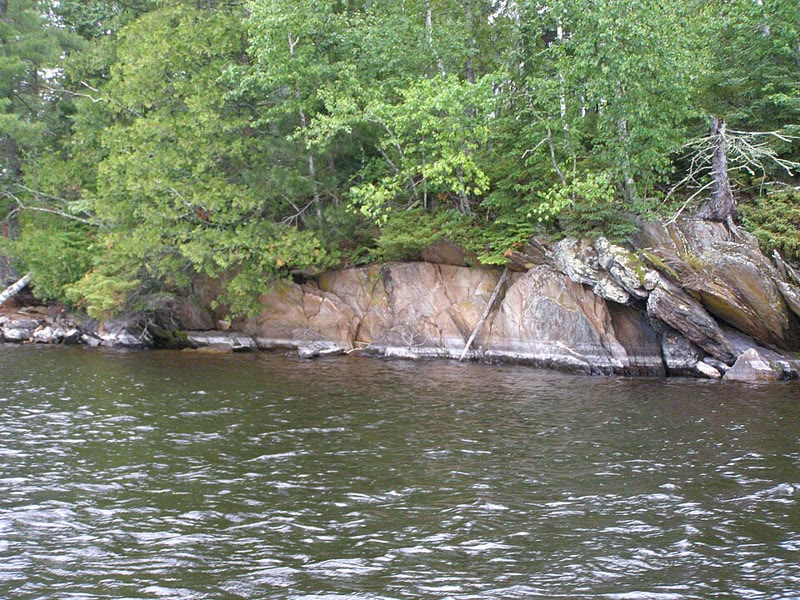
\includegraphics[height=5.0cm]{images/book2/g12-light-canadian-shield.jpg}

{\small 湖岸边年龄为 10 亿至 30 亿年的片麻岩和花岗岩，
位于加拿大，是北美古老核心的一部分。照片：Chris Light
（CC~BY-SA~4.0）。}
\end{omfigure}
% ledger: photo:g12-canadian-shield

为什么\omterm{def:g12:continental-crust:continental-crust}{大陆地壳}能够长期存在，而洋底总是年轻的？
\omterm{def:g11:ocean-ridges:oceanic-lithosphere}{洋壳}密度大，在\omterm{def:g11:subduction-zones:subduction}{俯冲带}下沉回到地幔中，
几乎没有哪部分能存留超过 2 亿年。\omterm{def:g12:continental-crust:continental-crust}{大陆
地壳}太轻而无法下沉；它可被侵蚀、拉伸或挤皱，
但始终留在地表。大陆的岩石是
一部长达四十亿年的档案。
% ledger: tulane:no-subduct, tulane:roots, data:b2-seafloor-age

\section{山根}

山越高，其下方的地壳越厚。

\begin{definition}[山根]\label{def:g12:continental-crust:root}
称\emph{山根}\index{山根（山脉）}为山脉的
增厚地壳中向下伸入地幔、深于周围低地之下
\omterm{def:g11:seismic-structure:moho}{莫霍面}的部分。
\end{definition}
% ledger: tulane:roots

艾里模型可预测\omterm{def:g12:continental-crust:root}{山根}：高出周围地面 $h$ 的山脉
其\omterm{def:g12:continental-crust:root}{山根} $r = h\,\rho_c/(\rho_m - \rho_c)$，约为其高度的五倍，
取 $\rho_c = \qty{2830}{kg/m^3}$ 和 $\rho_m =
\qty{3380}{kg/m^3}$（见\cref{prop:g11:lithosphere-asthenosphere:airy}）。两类
测量可探测\omterm{def:g12:continental-crust:root}{山根}。地震测量表明，\omterm{def:g11:seismic-structure:moho}{莫霍面}在山脉之下更深：许多山带之下
深约 50 至 \qty{70}{km}，西藏部分地区约为
\qty{70}{km}。山脉上方的重力比其可见质量所暗示的要弱：
轻质的\omterm{def:g12:continental-crust:root}{山根}占据了本应是较重地幔的位置，
在深部造成质量亏损，实测的重力异常随地形
及地震学测得的地壳厚度而变化。大陆漂浮，
其上的山脉漂浮得最高。
% ledger: tulane:roots, karplus:tibet-moho, cm95:crust, data:prem

\section{练习}

\begin{exercise}[$\star$]\label{exo:g12:continental-crust:1}
抄写并补全下表，比较\omterm{def:g12:continental-crust:continental-crust}{大陆地壳}与\omterm{def:g11:ocean-ridges:oceanic-lithosphere}{洋壳}的厚度；
主要岩石；二氧化硅含量；密度；最大年龄。
\end{exercise}

\begin{exercise}[$\star$]\label{exo:g12:continental-crust:2}
整个\omterm{def:g12:continental-crust:continental-crust}{大陆地壳}含二氧化硅 \qty{60.6}{\percent}，其上部
含 \qty{66.6}{\percent}。根据火成岩的二氧化硅分类，
判断两者各为\omterm{def:g11:igneous-rocks:felsic-mafic}{镁铁质}、\omterm{def:g11:igneous-rocks:felsic-mafic}{中性}还是\omterm{def:g11:igneous-rocks:felsic-mafic}{长英质}，
并写出一种成分相同的\omterm{def:g11:igneous-rocks:volcanic-plutonic}{深成岩}的名称。
\end{exercise}

\begin{exercise}[$\star$]\label{exo:g12:continental-crust:3}
为什么\omterm{def:g11:ocean-ridges:oceanic-lithosphere}{洋壳}能在\omterm{def:g11:subduction-zones:subduction}{俯冲带}沉入地幔，而\omterm{def:g12:continental-crust:continental-crust}{大陆地壳}不能？
请用密度作答。
\end{exercise}

\begin{exercise}[$\star$]\label{exo:g12:continental-crust:4}
(1) 什么是\omterm{def:g12:continental-crust:craton}{克拉通}？(2) \omterm{def:g12:continental-crust:craton}{克拉通}的岩石至少有多老？
(3) 它由哪些种类的岩石组成？
\end{exercise}

\begin{exercise}[$\star$]\label{exo:g12:continental-crust:5}
最古老的洋底约为 1.9 亿年，阿卡斯塔片麻岩为 40.3 亿年。
片麻岩的年龄是洋底的多少倍？为什么没有
同样古老的洋底？
\end{exercise}

\begin{exercise}[$\star\star$]\label{exo:g12:continental-crust:6}
\omterm{def:g12:continental-crust:continental-crust}{大陆地壳}覆盖面积为 2.104 亿~\unit{km^2}，其中
\qty{30.6}{\percent} 位于海下。(1) 位于海下的\omterm{def:g12:continental-crust:continental-crust}{大陆地壳}面积是多少？
(2) 高出海面的面积是多少？(3) 地球表面积为
$4\pi R^2$，其中 $R = \qty{6371}{km}$。\omterm{def:g12:continental-crust:continental-crust}{大陆地壳}覆盖的
面积占地表面积的比例是多少？
\end{exercise}

\begin{exercise}[$\star\star$]\label{exo:g12:continental-crust:7}
计算截面积为 \qty{1}{m^2} 的一段地壳柱体的质量，
从地表到\omterm{def:g11:seismic-structure:moho}{莫霍面}：(1) 穿过 \qty{41.1}{km} 的\omterm{def:g12:continental-crust:continental-crust}{大陆地壳}，
密度为 \qty{2830}{kg/m^3}；(2) 穿过 \qty{7.1}{km} 的\omterm{def:g11:ocean-ridges:oceanic-lithosphere}{洋壳}，密度为
\qty{3000}{kg/m^3}。(3) 第一种的质量是第二种的多少倍？
\end{exercise}

\begin{exercise}[$\star\star$]\label{exo:g12:continental-crust:8}
某山脉比地壳厚 \qty{35}{km} 的低地高出 \qty{2.5}{km}，
设 $\rho_c = \qty{2830}{kg/m^3}$，$\rho_m =
\qty{3380}{kg/m^3}$，求其\omterm{def:g12:continental-crust:root}{山根}的深度和地壳厚度。
所得结果是否落在造山带下实测的范围内？
\end{exercise}

\begin{exercise}[$\star\star$]\label{exo:g12:continental-crust:9}
根据洋底年龄直方图，(1) 年龄小于 3000 万年的洋底占
比例为多少？(2) 哪个 1000 万年的年龄区间所含洋底最多？
(3) 为什么占比随年龄增大而下降？
\end{exercise}

\begin{exercise}[$\star\star$]\label{exo:g12:continental-crust:10}
连同海下部分一并统计时，\omterm{def:g12:continental-crust:continental-crust}{大陆地壳}的平均高度
约为 \qty{120}{m}。设海下部分占其面积的 \qty{30.6}{\percent}，
平均位于海平面下 \qty{100}{m}。其露出部分的
平均高度是多少？为什么早期只统计陆地的估计会得出高得多的
平均高度？
\end{exercise}

\begin{exercise}[$\star\star$]\label{exo:g12:continental-crust:11}
一个位于远海岛屿上的钻孔，在几百米厚的
熔岩之下钻遇\omterm{def:g11:ocean-ridges:gabbro}{辉长岩}；地震剖面显示\omterm{def:g11:seismic-structure:moho}{莫霍面}位于地下 \qty{8}{km}。
另一钻孔位于广阔平坦的平原上，在 \qty{2}{km} 深处钻遇片麻岩，
\omterm{def:g11:seismic-structure:moho}{莫霍面}位于地下 \qty{38}{km}。运用该方法判断
两处分别位于何种地壳之下。
\end{exercise}

\begin{exercise}[$\star\star\star$]\label{exo:g12:continental-crust:12}
命题中的近似有多好？(1) 计算半径为 \qty{6371}{km} 的球面
表层、厚度为 \qty{41.1}{km} 的壳层的精确体积
$\tfrac{4}{3}\pi\bigl(R^3 - (R - H)^3\bigr)$，以及近似体积
$4\pi R^2 H$。(2) 二者的相对差是多少？
将其与 $H/R$ 比较。
\end{exercise}

\begin{exercise}[$\star\star\star$]\label{exo:g12:continental-crust:13}
设\omterm{def:g12:continental-crust:continental-crust}{大陆地壳}按质量计的上部三分之一含二氧化硅
\qty{66.6}{\percent}，整个地壳含 \qty{60.6}{\percent}。(1)
下部三分之二的二氧化硅含量是多少？(2) 它与哪一类火成岩
相符？(3) 这说明深部\omterm{def:g12:continental-crust:continental-crust}{大陆地壳}
有何性质？
\end{exercise}

\begin{exercise}[$\star\star\star$]\label{exo:g12:continental-crust:14}
设洋脊处每年新生\omterm{def:g11:ocean-ridges:oceanic-lithosphere}{洋壳}约 \qty{3}{km^2}，
而洋底面积约为 3 亿~\unit{km^2}。(1)
洋脊需要多长时间才能生成与整个洋底面积相等的\omterm{def:g11:ocean-ridges:oceanic-lithosphere}{洋壳}？
(2) 将结果与洋底年龄比较。(3) 古老的洋底
必然发生什么？
\end{exercise}

\begin{exercise}[$\star\star\star$]\label{exo:g12:continental-crust:15}
设全部\omterm{def:g12:continental-crust:continental-crust}{大陆地壳} \qty{8.6e9}{km^3} 自 40 亿年前起
以恒定速率形成。(1) 以立方千米每年计算该速率。
(2) 杰克山的锆石表明，早在
44 亿年前已有部分地壳存在。恒定速率是否符合大部分地壳
可能形成于早期还是晚期的世界？最古老的岩石能说明什么，
又不能说明什么，考虑到古老地壳可能被侵蚀或再循环？
\end{exercise}

\section{问题：大陆地壳有多重？}

\begin{problem}[{周末问题——大陆的质量}]
\label{pb:g12:continental-crust:1}
% ledger: cogley84:continents, cm95:crust, earth:mass, earth:Rmean, earth:density, white92:crust
% values: 4 pi R^2 = 5.1006e8 km2; V = 210.4e6 x 41.1 = 8.647e9 km3; m = 2.447e22 kg; m/M = 0.410 %
\omterm{def:g12:continental-crust:continental-crust}{大陆地壳}覆盖面积为 2.104 亿~\unit{km^2}（包括
海下部分）。地震测量给出其平均厚度为 \qty{41.1}{km}，
平均密度为 \qty{2830}{kg/m^3}。地球平均半径为
\qty{6371}{km}，质量为 \qty{5.9722e24}{kg}，平均密度为
\qty{5513}{kg/m^3}。

\medskip
\noindent\textbf{第一部分——面积。}
\begin{enumerate}
  \item 计算地球表面积 $4\pi R^2$，单位为
        \unit{km^2}。
  \item \omterm{def:g12:continental-crust:continental-crust}{大陆地壳}覆盖了其中的多大比例？
  \item \omterm{def:g12:continental-crust:continental-crust}{大陆地壳}的 \qty{30.6}{\percent} 位于海下。
        该部分面积是多少？
  \item 假设其余地表全部为\omterm{def:g11:ocean-ridges:oceanic-lithosphere}{洋壳}，地表中留给
        \omterm{def:g11:ocean-ridges:oceanic-lithosphere}{洋壳}的面积是多少？
  \item 为什么\omterm{def:g12:continental-crust:continental-crust}{大陆地壳}的面积大于陆地面积？
\end{enumerate}

\medskip
\noindent\textbf{第二部分——厚度与体积。}
\begin{enumerate}[resume]
  \item 为什么仍可用面积乘以厚度计算体积，
        尽管地壳位于球面上？
  \item 计算\omterm{def:g12:continental-crust:continental-crust}{大陆地壳}的体积，单位为 \unit{km^3}。
  \item 将其换算为 \unit{m^3}。
  \item 平均厚度的另一种估计为 \qty{36}{km}，
        此时的体积是多少？
  \item 两个体积相差百分之多少？
\end{enumerate}

\medskip
\noindent\textbf{第三部分——密度与质量。}
\begin{enumerate}[resume]
  \item 取厚度为 \qty{41.1}{km}，计算\omterm{def:g12:continental-crust:continental-crust}{大陆地壳}的质量。
  \item 计算穿过\omterm{def:g12:continental-crust:continental-crust}{大陆地壳}的柱体的质量，
        该柱体底面积为 \qty{1}{m^2}。
  \item 计算\omterm{def:g11:ocean-ridges:oceanic-lithosphere}{洋壳}的质量：面积取第 4 题的结果，
        厚度为 \qty{7.1}{km}，密度为 \qty{3000}{kg/m^3}。
  \item 哪一个更重？重多少倍？
        虽然其覆盖面积较小，原因何在？
  \item 为什么\omterm{def:g12:continental-crust:continental-crust}{大陆地壳}的密度小于\omterm{def:g11:ocean-ridges:oceanic-lithosphere}{洋壳}的密度？
\end{enumerate}

\medskip
\noindent\textbf{第四部分——与地球的比较。}
\begin{enumerate}[resume]
  \item 用第 11 题的质量除以地球的质量。
  \item 用关于薄层的命题检验结果。
  \item \omterm{def:g11:ocean-ridges:oceanic-lithosphere}{洋壳}的质量占地球质量的多大比例？
  \item \omterm{def:g12:continental-crust:continental-crust}{大陆地壳}保存着仅有的、早于约
        2 亿年的岩石。占地球质量多大比例的部分
        保存了其几乎全部历史的记录？
  \item 总结：\omterm{def:g12:continental-crust:continental-crust}{大陆地壳}的质量占地球质量的多大比例？
\end{enumerate}
\end{problem}
